% Copyright 2004 by Till Tantau <tantau@users.sourceforge.net>.
%
% In principle, this file can be redistributed and/or modified under
% the terms of the GNU Public License, version 2.
%
% However, this file is supposed to be a template to be modified
% for your own needs. For this reason, if you use this file as a
% template and not specifically distribute it as part of a another
% package/program, I grant the extra permission to freely copy and
% modify this file as you see fit and even to delete this copyright
% notice. 

\documentclass[11pt]{beamer}
\usepackage[rightcaption]{sidecap}
 
\usepackage{graphicx}
\graphicspath{}

\usepackage[backend=biber,
    style=numeric,]{biblatex}
\addbibresource{Reference.bib}

% There are many different themes available for Beamer. A comprehensive
% list with examples is given here:
% http://deic.uab.es/~iblanes/beamer_gallery/index_by_theme.html
% You can uncomment the themes below if you would like to use a different
% one:
%\usetheme{AnnArbor}
%\usetheme{Antibes}
%\usetheme{Bergen}
%\usetheme{Berkeley}
%\usetheme{Berlin}
%\usetheme{Boadilla}
%\usetheme{boxes}
%\usetheme{CambridgeUS}
%\usetheme{Copenhagen}
%\usetheme{Darmstadt}
%\usetheme{default}
%\usetheme{Frankfurt}
%\usetheme{Goettingen}
%\usetheme{Hannover}
%\usetheme{Ilmenau}
%\usetheme{JuanLesPins}
%\usetheme{Luebeck}
\usetheme{Madrid}
%\usetheme{Malmoe}
%\usetheme{Marburg}
%\usetheme{Montpellier}
%\usetheme{PaloAlto}
%\usetheme{Pittsburgh}
%\usetheme{Rochester}
%\usetheme{Singapore}
%\usetheme{Szeged}
%\usetheme{Warsaw}
%\newcommand{\dag}{\dagger}
\title{\textbf{Graphene : Spin-Orbit Coupling}}

% A subtitle is optional and this may be deleted
\subtitle{EP  : Course Seminar}

\author[Sanket Chirame]{Sanket Chirame \\ 14D260003}
% - Give the names in the same order as the appear in the paper.
% - Use the \inst{?} command only if the authors have different
%   affiliation.

%\institute[IIT Bombay] % (optional, but mostly needed)
%{ Department of Physics\\
 % IIT Bombay
 % }
% - Use the \inst command only if there are several affiliations.
% - Keep it simple, no one is interested in your street address.

%\date[SLP Autumn 2016]{Supervised Learning Project \\ 
%Autumn 2016}
% - Either use conference name or its abbreviation.
% - Not really informative to the audience, more for people (including
%   yourself) who are reading the slides online

%\subject{Theoretical Computer Science}
% This is only inserted into the PDF information catalog. Can be left
% out. 

% If you have a file called "university-logo-filename.xxx", where xxx
% is a graphic format that can be processed by latex or pdflatex,
% resp., then you can add a logo as follows:

% \pgfdeclareimage[height=0.5cm]{university-logo}{university-logo-filename}
% \logo{\pgfuseimage{university-logo}}

% Delete this, if you do not want the table of contents to pop up at
% the beginning of each subsection:
%\AtBeginSubsection[]
%{
%  \begin{frame}<beamer>{Outline}
%    \tableofcontents[currentsection,currentsubsection]
%  \end{frame}
%}

\begin{document}
\begin{frame}
  \titlepage 
\end{frame}
\begin{frame}{Intrinsic Spin-Orbit splitting}
\begin{itemize}
    \item Interaction arises due to coupling of internal potential with spin of electrons
    \item Effective Hamiltonian:
    \[\ H_{SO} = \lambda_I \kappa\sigma_zs_z \]
    \item Here, $s_z$  : Pauli spin matrix in the electron-spin space
    \item The dispersion relation for total Hamiltonian $H_0+H_{SO}$ is
    \[\ \epsilon_\nu = \nu\sqrt{\epsilon_0^2+\lambda_I^2} \]
    \item The space inversion and Time reversal symmetries
    \item Two fold degeneracy in bands
\end{itemize}
\end{frame}
\begin{frame}{Intrinsic Spin-Orbit splitting}
\begin{figure}[h]
    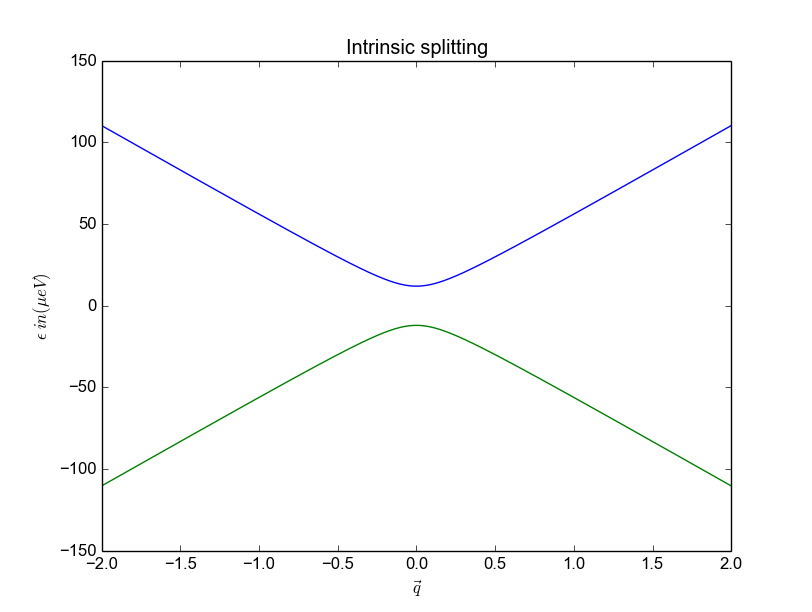
\includegraphics[height=0.3\textwidth,width = .5\textwidth]{figure_1}
    \caption{Intrinsic Spin-orbit splitting}
\end{figure}
The energy gap of $|2\lambda_I|$ opens at the Dirac points.\\
Conical shape is replaced by smooth curvature.
\end{frame}
\begin{frame}{Extrinsic Spin-orbit splitting}.
\begin{itemize}
    \item In the presence of transverse electric field,
\[\ H_{BR} = \lambda_{BR}(\kappa\sigma_xs_y -\sigma_ys_x ) \]
    \item $\lambda_{BR}$ : Bychkov-Rashba parameter
    \item The energy-momentum dispersion relation is given by
    \[\ \epsilon_{\mu\nu} = \mu\lambda_{BR} + \nu\sqrt{(\hbar\nu_Fk)^2 + (\lambda_{BR} - \mu\lambda_I)^2} \]
    \item The degeneracy is lifted except at Dirac points
    \item $\lambda_{BR}$ depends upon the strength of applied electric field.
\end{itemize}
\end{frame}
\begin{frame}{$\lambda_{BR}<\lambda_I$}
\begin{figure}[h]
    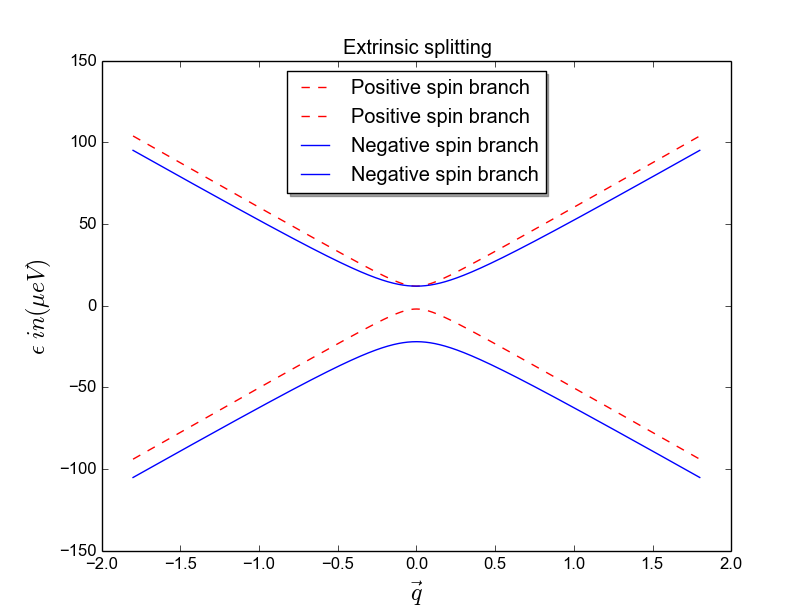
\includegraphics[height=0.3\textwidth,width = .5\textwidth]{figure_2}
    \caption{Extrinsic Spin-orbit splitting when $E = 1.0 V/nm$}
\end{figure}
\end{frame}
\begin{frame}{$\lambda_{BR}=\lambda_I$}
\begin{figure}[h]
    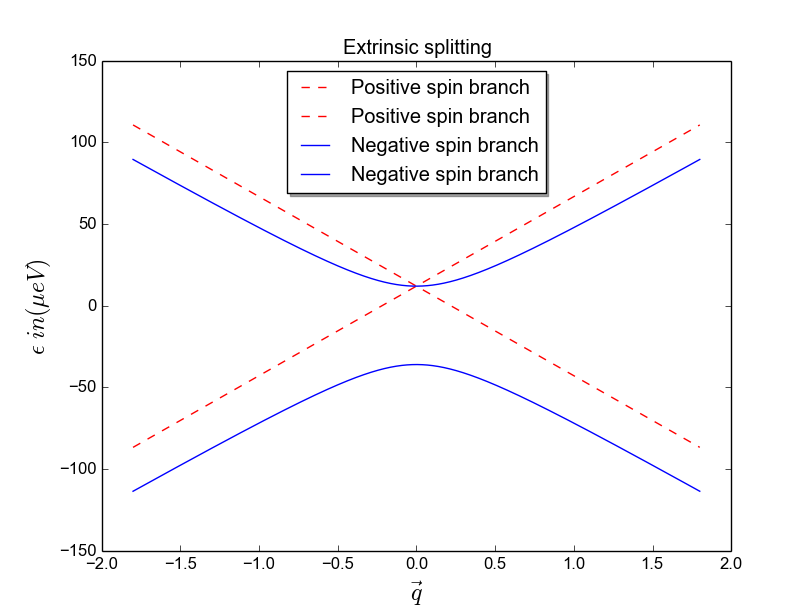
\includegraphics[height=0.3\textwidth,width = .5\textwidth]{figure_3}
    \caption{Extrinsic Spin-orbit splitting when $E = 2.44 V/nm$}
\end{figure}
\begin{itemize}
    \item Positive spin branches form massless fermion like cone.
    \item The remaining branches are massive parabolic bands.
\end{itemize}

\end{frame}
\begin{frame}{$\lambda_{BR}>\lambda_I$}
\begin{figure}[h]
    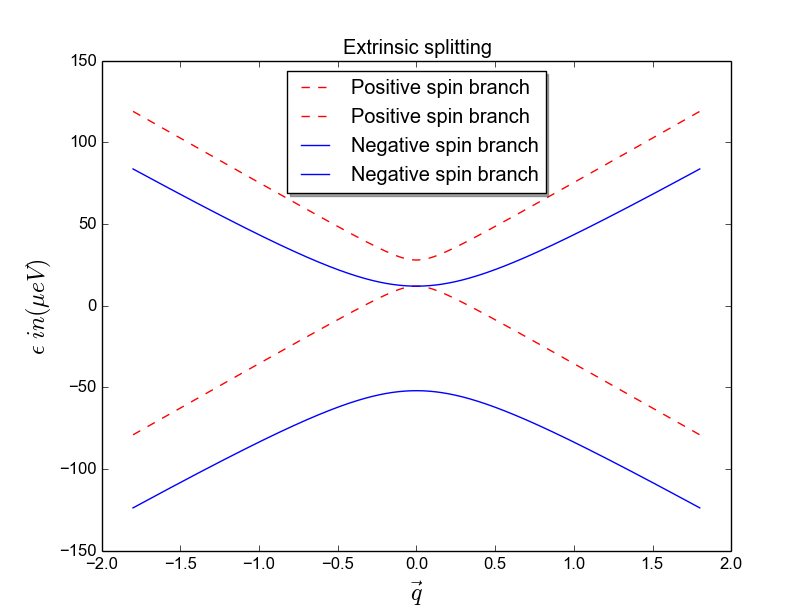
\includegraphics[height=0.3\textwidth,width = .5\textwidth]{figure_4}
    \caption{Extrinsic Spin-orbit splitting when $E = 4 V/nm$}
\end{figure}
\end{frame}
\begin{frame}{Modification in Intrinsic splitting}
The authors propose that the value of $2\lambda_I$ is $24 \mu eV$. Whereas the earlier reported value is around $1\mu eV.$
\begin{itemize}
    \item Previous result were not truly from first principle calculations.
    \item The contribution from $d$ and higher orbitals are also taken into account.
    \item The contribution from $s,p$ is lower compared to $d$.
    \item Removing the contribution of $d$ orbitals gives back the old results.
\end{itemize}
\begin{figure}[h]
    \includegraphics[height=0.3\textwidth,width = .5\textwidth]{figure_5}
    \caption{Projected density of states to particular atomic orbitals}
\end{figure}

\end{frame}
\begin{frame}{References}
\printbibliography
\end{frame}
\end{document}


